\section{Requisiti}

Si vuole realizzare un sistema software completo che offrirà agli utenti un servizio di sharing musicale 
integrato con le funzionalità di un social network. L'obiettivo principale è fornire agli utenti un'esperienza 
musicale coinvolgente, consentendo loro di esplorare nuovi brani, condividere le proprie preferenze musicali e 
connettersi con artisti e amici che condividono interessi simili.

Durante la fase di registrazione, agli utenti verrà richiesto di inserire le proprie informazioni personali, 
come nome, compleanno, e altri dettagli pertinenti. Queste informazioni saranno utilizzate per personalizzare 
l'esperienza musicale di ciascun utente.

Una volta registrati, l'algoritmo del sistema entrerà in azione. Utilizzando le informazioni fornite dagli utenti 
durante la registrazione, l'algoritmo analizzerà le preferenze musicali e suggerirà loro i brani più popolari e 
rilevanti basati su tali preferenze. Questo consentirà agli utenti di scoprire nuove canzoni e artisti che potrebbero interessarli.

Oltre a suggerire brani, il sistema offrirà anche la possibilità di esplorare le affinità musicali. 
Gli utenti potranno visualizzare le playlist e i gusti musicali dei propri amici e scoprire artisti 
correlati in base alle preferenze comuni. Ciò favorirà l'interazione sociale tra gli utenti e creerà
 un ambiente in cui gli appassionati di musica potranno connettersi, scoprire nuove tracce e condividere le proprie esperienze musicali.

Nel sistema saranno coinvolti due principali attori:  
\begin{itemize}
      \item \textbf{Utenti:} coloro che desiderano ascoltare musica, conoscere nuovi artisti e condividere 
      le proprie attività musicali con gli amici;
      \item \textbf{Artisti:} sia indipendenti che facenti parte di case discografiche, che desiderano 
      pubblicare e gestire la propria musica sul sistema.
\end{itemize}

In questo modo, gli artisti potranno raggiungere un pubblico più vasto e gli utenti avranno accesso a una vasta gamma 
di brani provenienti da artisti diversi.

Complessivamente, il sistema software offrirà una piattaforma interattiva e coinvolgente per gli amanti della musica, 
consentendo loro di esplorare, condividere e connettersi attraverso la passione comune per la musica.

Per poter accedere ai servizi offerti dal sistema, l'utente dovrà effettuare una registrazione e creare un proprio profilo personale. 
Una volta completata la registrazione, l'utente verrà indirizzato alla homepage del sistema, dove avrà accesso a diverse funzionalità.

Sulla \textbf{homepage}, l'utente potrà visualizzare i brani che ha apprezzato e le proprie playlist personalizzate. 
Avrà la possibilità di effettuare ricerche specifiche per trovare brani desiderati e potrà anche accedere alla 
sezione delle impostazioni personali e social, per personalizzare il proprio profilo e le preferenze di condivisione.

Quando l'utente seleziona un brano per il \textbf{download}, il sistema fornirà tutte le informazioni relative ad esso, 
come il titolo, l'artista, l'album e il genere di appartenenza. Questo permetterà all'utente di ottenere una panoramica 
completa del brano prima di procedere al download.

Il software offre anche la possibilità di mettere \textbf{``like''} ai brani e creare playlist personalizzate. 
Nella libreria musicale dell'utente saranno quindi presenti le sue playlist personali e una lista dei brani preferiti. 
Questo consentirà all'utente di organizzare la propria musica in base ai propri gusti e preferenze.

Inoltre, l'interfaccia sociale del sistema permette all'utente di aggiungere \textbf{amici}. 
Ciò consente di connettersi con altre persone che condividono interessi musicali simili e facilita 
la condivisione di brani, playlist e esperienze musicali tra amici.

La funzionalità principale offerta dal servizio è l'\textbf{algoritmo ``Discover"}, progettato per consentire 
agli utenti di trovare i brani più apprezzati da altre persone che condividono gli stessi generi musicali di interesse. 
Questo algoritmo è fondamentale per permettere agli utenti di scoprire sempre nuove canzoni e ampliare il 
loro repertorio musicale. Grazie all'algoritmo "Discover", gli utenti potranno esplorare un vasto catalogo musicale e 
ricevere raccomandazioni personalizzate basate sui loro gusti musicali.

Inoltre, l'algoritmo non solo suggerirà nuove canzoni, ma sarà anche in grado di proporre nuovi amici 
con gusti musicali affini. Questo incoraggerà l'interazione sociale all'interno della piattaforma, consentendo 
agli utenti di connettersi con altre persone che condividono le loro preferenze musicali e facilitando la scoperta e 
la condivisione di brani e playlist tra amici.

Per quanto riguarda gli artisti, il servizio offre loro la possibilità di caricare brani singoli e album. 
Gli artisti potranno inserire i dati relativi alla propria produzione artistica, come titolo, artista, album e 
altre informazioni pertinenti. Questo permetterà loro di pubblicare e gestire la propria musica all'interno 
della piattaforma, raggiungendo un pubblico più vasto e offrendo agli utenti la possibilità di scoprire e ascoltare la loro musica.



\vspace{1cm}
\section{Studio di fattibilità}
Procedendo con una valutazione dei costi e dei benefici della possibile realizzazione del
presente sistema, è possibile concludere che i costi principali sono relativi alla
funzionalità di Discover e brani consigliati. 

Per realizzare questa funzionalità è
necessaria l'implementazione di un algoritmo che vada a studiare i gusti e le preferenze
di ogni singolo utente e, dopo la preliminare fase di raccolta dati, proporrà all'utente
una serie di brani in linea con le sue preferenze. 

Per quanto riguarda invece la
fattibilità in termini di tecnologie e strumenti per la realizzazione del sistema 
il costo principale da considerare è quello relativo allo sviluppo del software e il servizio di hosting sia 
della piattaforma che del database. 


\newpage
\section{Casi d'uso}
Di seguito vengono riportati i casi d'uso raggruppati in base all'attore coinvolto. Come
anticipato gli attori in gioco sono i seguenti:
\begin{itemize}
      \item Utente ascoltatore;
      \item Artista;
\end{itemize}

\vspace{0.5cm}
\subsection{Casi d'uso utente}
\begin{itemize}
      \item \textbf{UC1: Sign up} 
            
      L'utente può registrarsi inserendo le sue informazioni personali.
      \item \textbf{UC2: Sign in}
      
      L'utente può accedere al proprio profilo personale inserendo nome utente e password.
      \item \textbf{UC3: Sign out} 
      
      L'utente può disconnettere il proprio profilo personale dal sistema.     
      \item \textbf{UC4: Cerca brano}
      
      L'utente può digitare nella barra di ricerca per cercare un brano dal titolo.
      \item \textbf{UC5: Cerca album}
      
      L'utente può digitare nella barra di ricerca per cercare un album dal titolo.
      \item \textbf{UC6: Cerca Artista}
      
      L'utente può digitare nella barra di ricerca per cercare un artista dal nome.
      \item \textbf{UC7: Scarica brano}
      
      L'utente può scaricare il brano.
      \item \textbf{UC8: Like al brano} 
      
      L'utente può esprimere il proprio interesse per un brano mettendo like.
      \item \textbf{UC9: Aggiungi brano a playlist}
      
      L'utente può aggiungere alla lista di brani della playlist un brano selezionato.
      \item \textbf{UC10: Cerca Utente} 
      
      L'utente può cercare un utente per nome dalla barra di ricerca apposita (cerca album/artista).
      \item \textbf{UC11: Aggiungi Utente} 
      
      L'utente può aggiungere alla propria lista amici un utente selezionato.
      \item \textbf{UC12: Visualizza informazioni profilo} 
      
      L'utente può consultare le proprie informazioni personali inserite in fase di registrazione.
      \item \textbf{UC13: Modifica profilo} 
      
      L'utente può modificare le proprie informazioni personali inserite in fase di registrazione.
      \item \textbf{UC14: Elimina profilo} 
      
      L'utente può eliminare il proprio profilo dal sistema.
      \item \textbf{UC15: Visualizza playlist} 
      
      L'utente può consultare tutte le proprie playlist.
      \item \textbf{UC16: Crea nuova playlist} 
      
      L'utente può creare una nuova playlist nella quale aggiungere brani.
      \item \textbf{UC17: Elimina playlist}
      
      L'utente può eliminare una delle proprie playlist.
      \item \textbf{UC18: Modifica playlist} 
      
      L'utente può modificare una delle proprie playlist, per esempio modificando il nome o rimuovendo brani.
      \item \textbf{UC19: ``Discover''} 
      L'utente può consultare brani scelti per lui dal sistema e amici suggeriti in base alle sue preferenze musicali.

\end{itemize}

\subsection{Casi d'uso artista}
\begin{itemize}
      \item \textbf{UC20: Crea pagina artista} 
      
      L'artista per poter pubblicare musica deve creare una pagina artista inserendo le proprie informazioni personali.
      \item  \textbf{UC21: Visualizza pagina artista} 
      
      L'artista può consultare la propria pagina artista, dove vengono visualizzati i propri brani/album pubblicati.
      \item  \textbf{UC22: Aggiungi brano} 
      
      L'artista può pubblicare un nuovo brano inserendo le informazioni relative.
      \item  \textbf{UC23: Aggiungi album} 
      
      L'artista può pubblicare un nuovo album contenente i brani scelti.
      \item  \textbf{UC24: Personalizza pagina artista} 
      
      L'artista può decidere quali brani e album mettere in evidenza nella propria pagina artista.
      \item  \textbf{UC25: Consulta anagrafica} 
      
      L'artista può consultare l'anagrafica relativa agli ascolti e ai like dei brani e album pubblicati.

\end{itemize}


\vspace{1cm}
\subsection{Dettaglio casi d'uso}
Di seguito verranno analizzati più nel dettaglio i casi d'uso sopra citati, 
identificandone descrizione, attore e passi principali.

Gli utenti avranno la possibilità di registrarsi al sito per poter fruire dei servizi di streaming di musica. 
Al momento della registrazione sarà necessario inserire alcune informazioni personali di base come nome, cognome, email. 
Inoltre si dovrà inserire un nome utente identificativo e una password, necessari per il login. Nel caso in cui l'utente 
sia già registrato sarà necessario inserire solo questi campi per accedere al sistema. 

Al termine dell'iscrizione è possibile navigare nella Home page, la quale si suddivide in varie sezioni. 

È possibile cercare un brano dalla barra di ricerca (tramite il titolo, nome dell'artista o nome 
dell'album) e scaricarlo.

Una volta scelto il brano, per ognuno di essi vengono visualizzate alcune informazioni come il titolo del brano, 
il nome dell'artista e l'etichetta discografica di riferimento.

È offerta la possibilità di mettere like al brano e creare playlist personalizzate con i propri brani preferiti: 
visualizzando la propria libreria, infatti, è possibile visualizzare i Brani Preferiti e le proprie playlist. 

Come anticipato il sistema offre anche funzionalità di un social network: infatti dalla barra di ricerca è possibile 
cercare per nome utente i propri amici e aggiungerli, in modo tale da poter condividere le proprie preferenze musicali. 

Una delle funzionalità principali offerte dal sistema è chiamata Discover e consiste nel poter usufruire di playlist 
create ad hoc dal sistema per l'utente, tramite lo studio delle sue preferenze. 

Gli artisti potranno gestire e pubblicare la propria musica tramite varie funzionalità offerte dal sistema. Al momento 
della registrazione bisogna seguire la procedura classica di sign-in, in seguito in una sezione apposita è offerta la 
possibilità di creare la pagina artista, all'interno della quale verrà inserito il nome che apparirà pubblicamente, 
insieme ad altre informazioni personali. 

Dopo aver creato il proprio profilo artista si potrà accedere alla propria pagina per pubblicare le proprie tracce, 
album, playlist, personalizzandola. Ogni volta che viene pubblicato un brano è possibile inserire eventuali nomi di 
collaboratori, artisti che hanno partecipato al brano e scrittori di testo e musica. Ogni artista può scegliere la 
data dalla quale rendere accessibile il brano o l'album.







\newpage
\subsection{Diagramma dei casi d'uso}

In figura \ref{fig-uml-use-cases} è stato riportato il diagramma dei casi d'uso, dove sono stati inseriti quelli
già precedentemente descritti mettendoli in correlazione con il corrispettivo attore.

\begin{figure}[H]
      \centering
      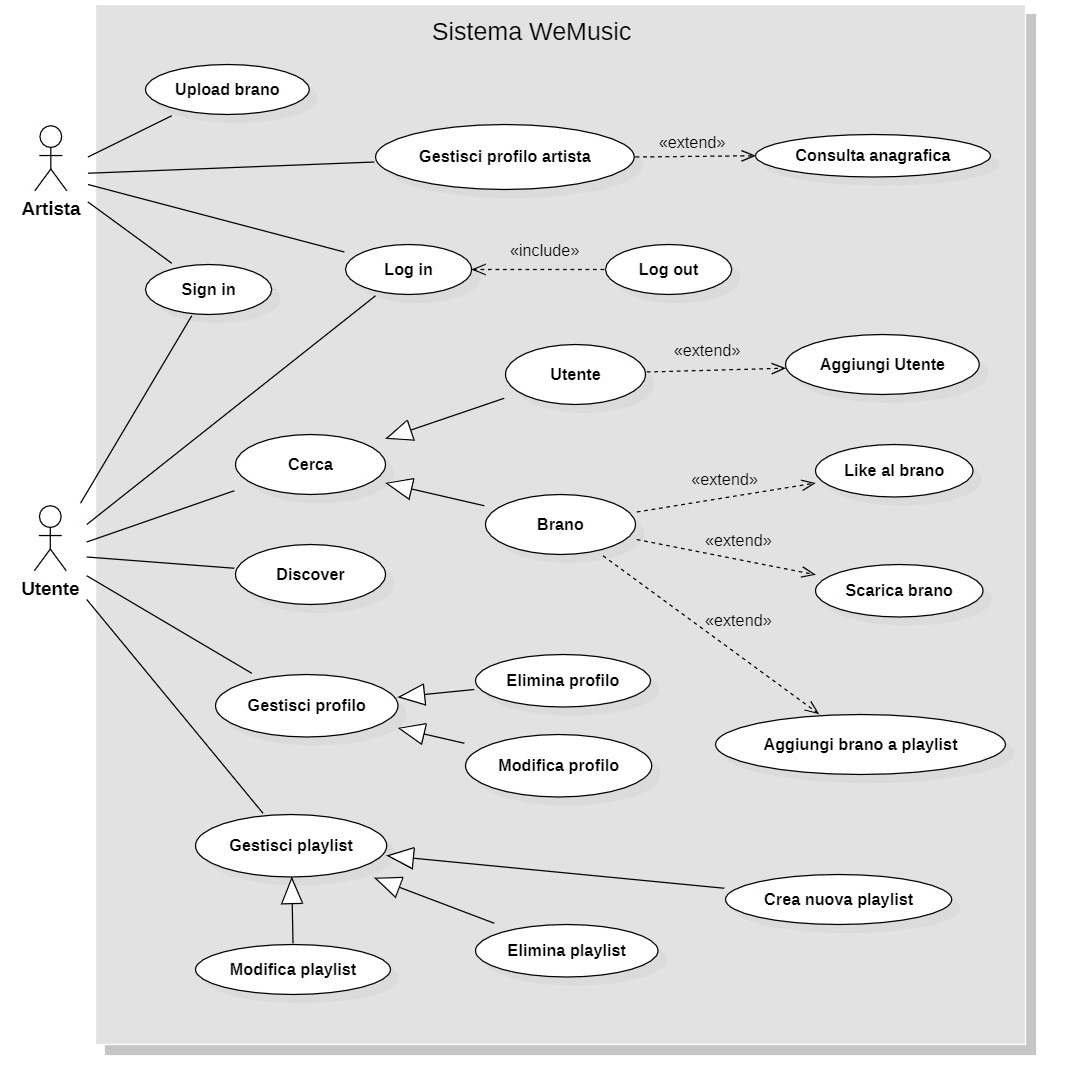
\includegraphics[scale=0.50]{UseCaseDiagram_ver4.jpg}
      \caption{UML Use Cases Diagram}
      \label{fig-uml-use-cases}
\end{figure}


\newpage
\section{Architettura del sistema}
L'architettura del sistema è stata formalizzata attraverso la rappresentazione tramite Deployment Diagram, diagramma di tipo statico 
sviluppato al fine di modellizzare e descrivere un sistema in termini di risorse hardware e di relazioni fra di esse.
Vengono sviluppati due Deployment Diagram differenti:

Il primo, riportato in figura \ref{architettura}, rappresenta il sistema
attraverso una notazione a stile libero, mentre il secondo, riportato in figura \ref{dep_diagram}, rappresenta
la topologia del sistema tramite lo stile UML. 

\vspace{2cm}

\subsection{Deployment diagram -- Informal}
In figura \ref{architettura} viene evidenziata la componente principale del sistema, il sistema gestore (WeMusic)
il Web Server (sviluppato tramite il framework Django) che, tramite una connessione ad internet, permette 
agli utenti di poter consultare il sito.
\begin{figure}[H]
      \centering
      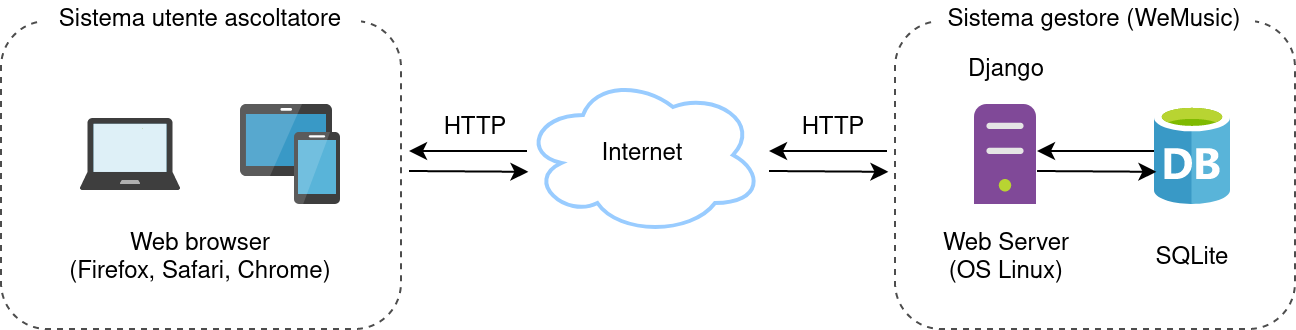
\includegraphics[width=\textwidth]{architettura.png}
      \caption{Architettura}
      \label{architettura}
\end{figure}


\newpage
\subsection{Deployment diagram -- UML}
In figura \ref{dep_diagram} vengono evidenziati due nodi principali: 
un lato client che gestirà il front-end del sistema WeMusic, e un lato server relativo 
al back-end e alla gestione del Database, in modo da velocizzare e semplificare l'interazione tra logica e dati. 
\begin{figure}[H]
    \centering
    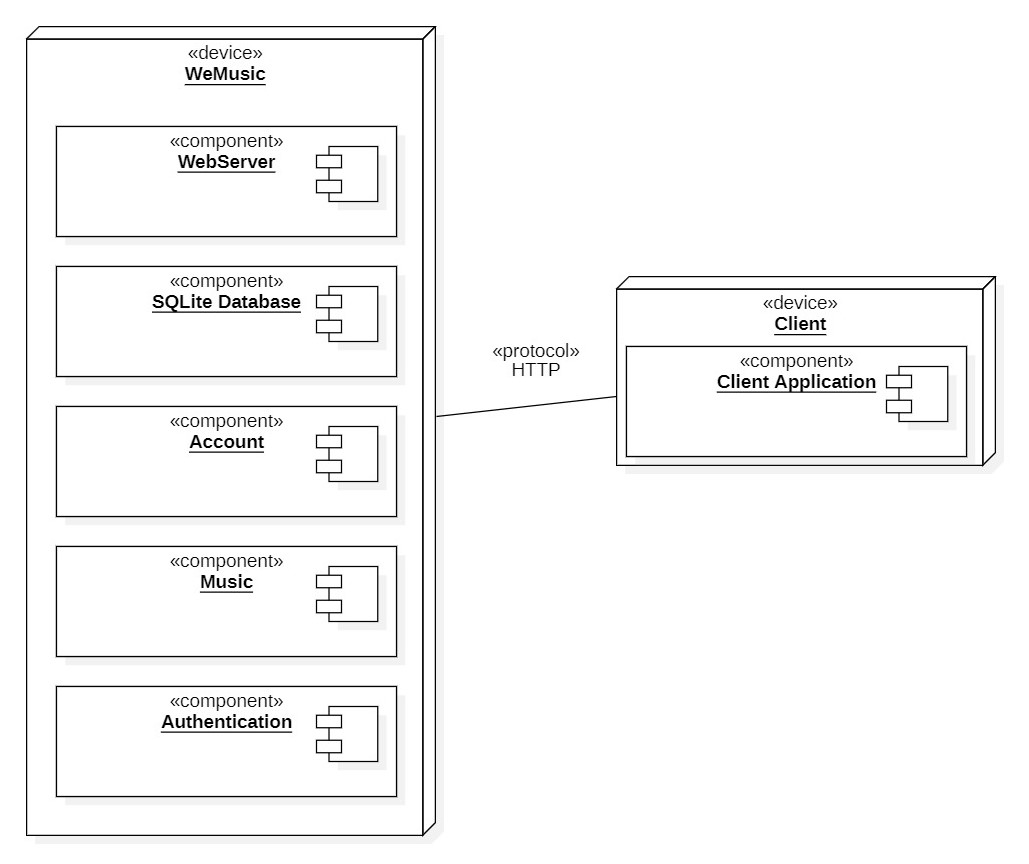
\includegraphics[width=\textwidth]{DeploymentDiagram_ver0.jpg}
    \caption{Deployment Diagram}
    \label{dep_diagram}
\end{figure}


